\documentclass[%
	11pt,
	a4paper,
	utf8,
	%twocolumn
		]{article}	

\usepackage{style_packages/podvoyskiy_article_extended}


\begin{document}
\title{Заметки по машинному обучению и анализу данных}

\author{{\itshape Подвойский Александр} 
\href{mailto:alexander.podvoyskiy@ipd.zyfra.com}{\ttfamily alexander.podvoyskiy@ipd.zyfra.com}\footnote{Комментарии и предложения приветствуются. Поругать автора можно по указанному адресу}}

\date{}
\maketitle

\thispagestyle{fancy}

Здесь будут собираться заметки по различным полезным инструментам разработки, техникам анализа и вычислительным приемам так или иначе затрагивающим вопросы машинного обучения и работу с данными


%\shorttableofcontents{Краткое содержание}{1}

\tableofcontents

\section{Инструмент управления git-публикациями \texttt{pre-commit}}

\subsection{Краткое описание}

\href{https://pre-commit.com/#new-hooks}{\ttfamily  pre-commit} -- это простой удобный инструмент управления git-хуками. Хук представляет собой пакет\footnote{Поддерживаются различные технологии: \texttt{bash}, \texttt{Python}, \texttt{dotenv}, \texttt{docker}, \texttt{ruby} etc.}, реализующий некоторую логику работы с зафиксированными изменениями кодовой базы до публикации этих изменений на удаленном сервере.

\texttt{pre-commit} поддерживает возможность создавать пользовательские хуки \url{https://pre-commit.com/#new-hooks}.

Установить инструмент можно, как обычно, с помощью менеджера пакетов \texttt{pip}
\begin{lstlisting}[
style = bash,
numbers = none	
]
pip install pre-commit
pre-commit install # установить pre-commit в git-хуки
\end{lstlisting}

После установки пакета \texttt{pre-commit} в командной оболочке будет доступна утилита командной строки с тем же именем.

Для того чтобы при фиксации изменений кодовой базы (\texttt{git commit}) запускалась цепочка проверок, следует в корне проекта разместить конфигурационный файл \texttt{.pre-commit-config.yaml}.

Типичный конфигурационный файл \texttt{pre-commit} управления git-хуками выглядит следующим образом
\begin{lstlisting}[
title = {\sffamily .pre-commit-config.yaml},
style = bash,
numbers = none
]
repos:
- repo: https://github.com/pre-commit/pre-commit-hooks
  rev: v4.0.1
  hooks:
  # проверяет наличие переноса строки в конце всех текстовых файлов
  - id: end-of-file-fixer
  # предупреждает о добавлении больших файлов в Git
  - id: check-added-large-files
  # предупреждает о сохранении файлов с UTF-8 BOM
  - id: fix-byte-order-marker
  # предотвращает сохранение приватных ключей
  - id: detect-private-key
  # убивает пробелы в конце строки
  - id: trailing-whitespace
  # проверяет на предмет расположения docstring после кода
  - id: check-docstring-first
  # проверяет файлы на предмет конфликтующих строк при операции слияния
  - id: check-merge-conflict
  # проводит синтаксический анализ yaml-файлов
  - id: check-yaml
  # проводит синтаксический анализ toml-файлов
  - id: check-toml
  # прводит синтаксический анализ json-файлов
  - id: check-json
- repo: https://github.com/pre-commit/mirrors-isort
  rev: f0001b2  # Use the revision sha / tag you want to point at
  hooks:
  - id: isort
    args: ["--profile", "black"]
- repo: https://github.com/psf/black
  rev: 21.7b0
  hooks:
    - id: black
    language_version: python3
- repo: https://github.com/asottile/yesqa
  rev: v1.1.0
  hooks:
    - id: yesqa
      additional_dependencies:
        - flake8-bugbear==20.1.4
        - flake8-builtins==1.5.2
        - flake8-comprehensions==3.2.2
        - flake8-tidy-imports==4.1.0
        - flake8==3.7.9
- repo: https://github.com/asottile/pyupgrade
  rev: v2.7.3
  hooks:
  - id: pyupgrade
    args: ['--py37-plus']
- repo: https://github.com/pre-commit/pygrep-hooks
  rev: v1.5.1
  hooks:
  - id: python-check-mock-methods
  - id: python-use-type-annotations

ci:
  autoupdate_commit_msg: 'chore: pre-commit autoupdate'
\end{lstlisting}

Теперь при каждой операции \texttt{git commit} будет запускаться цепочка проверок. Однако при желании эту цепочку можно запустить и без фиксации изменений, просто набрав в командной оболочке \verb|pre-commit run --all-files| (см.~\pic{fig:pre-commit-run}).

\begin{figure}[h]
	\centering
	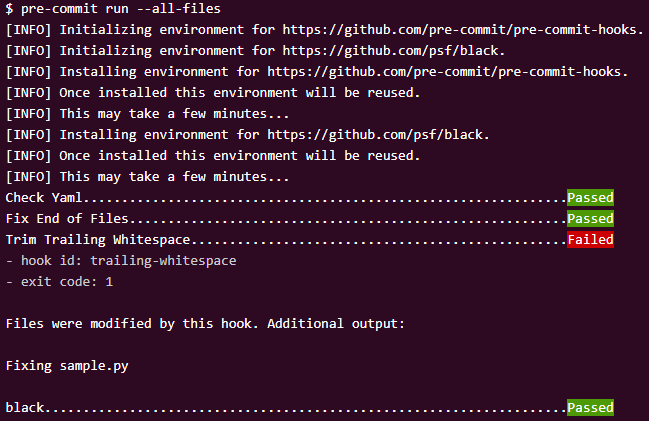
\includegraphics[scale=1.35]{figures/pre-commit-run.png}
	\caption{ Сеанс \texttt{pre-commit run} }\label{fig:pre-commit-run}
\end{figure}

Для управления настройками отдельных хуков (\texttt{flake8}, \texttt{black} и т.д.) в корне проекта можно разместить соответсвующие конфигурационные файлы.

Например, для \texttt{flake8}
\begin{lstlisting}[
title = {\sffamily .flake8},
style = bash,
numbers = none
]
[flake8]
  ignore =
    E402, W503 # для того, чтобы flake8 пропускал сообщения с этими метками
\end{lstlisting}

Для хука \texttt{isort}
\begin{lstlisting}[
title = {\sffamily .isort.cfg},
style = bash,
numbers = none
]
[tool.isort]
profile = "black"
multi_line_output = 3
include_tralling_comma = True
force_grid_wrap = 0
use_parenthese = True
ensure_newline_before_comments = True
line_length = 119
\end{lstlisting}

Для хука \texttt{black}
\begin{lstlisting}[
title = {\sffamily pyproject.toml},
style = bash,
numbers = none
]
# Example configuration for Black.

# NOTE: you have to use single-quoted strings in TOML for regular expressions.
# It's the equivalent of r-strings in Python.  Multiline strings are treated as
# verbose regular expressions by Black.  Use [ ] to denote a significant space
# character.

[tool.black]
line-length = 79
target-version = ['py36', 'py37', 'py38']
include = '\.pyi?$'
exclude = '''
/(
    \.eggs
  | \.git
  | \.hg
  | \.mypy_cache
  | \.tox
  | \.venv
  | _build
  | buck-out
  | build
  | dist
)/
'''
\end{lstlisting}

\subsection{Порядок работы}

В сухом остатке простейший шаблон работы с \texttt{pre-commit} выглядит так
\begin{itemize}
	\item либо цепочка проверок запускается через командную оболочку
\begin{lstlisting}[
style = bash,
numbers = none
]
pre-commit --version # pre-commit 2.14.0
pre-commit run --color always --all-files	# чтобы запустить все хуки
pre-commit run <hook_id> # если нужно запустить какой-то конкретный хук
pre-commit clean # очищает кэш
pre-commit gc # удаляет неиспользуемые репозитории кэш-каталога; рекомендуется выполнять эту команду время от времени
\end{lstlisting}

    \item либо автоматически <<за кадром>> при попытке фиксации изменений с помощью \texttt{git commit}
\end{itemize}

Убедиться в том, что \texttt{Git} использует не сценарий \texttt{pre-commit} по умолчанию, а тот сценарий, который создан пакетом \texttt{pre-commit} можно так
\begin{lstlisting}[
style = bash,
numbers = none	
]
cat .git/hooks/pre-commit | sed -n "/gener.*/p" # File generated by pre-commit: https://pre-commit.com
\end{lstlisting}


\subsection{Полезные ресурсы}

Сайт проекта \texttt{pre-commit}: \url{https://pre-commit.com/#plugins}.

Каталог хуков: \url{https://pre-commit.com/hooks.html}.

\section{Библиотека \texttt{csvkit} для работы с большими csv-файлами в командной оболочке}

\subsection{Краткое описание}

Иногда возникает необходимость \emph{быстро} провести разведочный анализ данных, представленных в виде <<больших>> (несколько сотен мегабайт) csv-файлов без необходимости привлекать специализированные библиотеки типа \texttt{pandas}, \texttt{dask}, \href{https://github.com/pola-rs/polars}{\ttfamily polars} и пр.

Утилита \href{https://github.com/wireservice/csvkit}{\ttfamily csvkit} как раз представляет собой такой инструмент командной строки.

Установить можно, как обычно с помощью, \texttt{pip}
\begin{lstlisting}[
style = bash,
numbers = none	
]
pip install csvkit
\end{lstlisting}

После установки пакета в командной облочке будут доступны следующие утилиты
\begin{itemize}
	\item \href{https://csvkit.readthedocs.io/en/latest/scripts/csvlook.html}{\ttfamily csvlook}: отвечает за <<human-readable>>-представление csv-файлов,
	
	\item \href{https://csvkit.readthedocs.io/en/latest/scripts/csvcut.html}{\ttfamily csvcut}: фильтрует и усекает csv-файлы (работает по аналогии с утилитой Linux \texttt{cut}),
	
	\item \href{https://csvkit.readthedocs.io/en/latest/scripts/in2csv.html}{\ttfamily in2csv}: преобразует различные табличные форматы, включая \texttt{*.xls(x)}, \texttt{*.geojson}, \texttt{*.dbf} и пр., в \texttt{*.csv},
	
	\item \href{https://csvkit.readthedocs.io/en/latest/scripts/csvstat.html}{\ttfamily csvstat}: возвращает описательные статистики для выбранных столбцов, 
	
	\item \href{https://csvkit.readthedocs.io/en/latest/scripts/csvgrep.html}{\ttfamily csvgrep}: отбирает строки, которые отвечают заданному условию или регулярному выражению,
	
	\item \href{https://csvkit.readthedocs.io/en/latest/scripts/csvsort.html}{\ttfamily csvsort}: сортирует csv-файлы (работает также как и Linux-аналог \texttt{sort}),
	
	\item \href{https://csvkit.readthedocs.io/en/latest/scripts/csvjoin.html}{\ttfamily csvjoint}: соединяет csv-файлы <<горизонтально>>,
	
	\item \href{https://csvkit.readthedocs.io/en/latest/scripts/csvstack.html}{\ttfamily csvstack}: соединяает csv-файлы <<вертикально>>,
	
	\item \href{https://csvkit.readthedocs.io/en/latest/scripts/csvsql.html}{\ttfamily csvsql}: выполняет SQL-запрос на csv-файле.
\end{itemize}


\subsection{Примеры использования}

Преобразование табличных форматов с заданной схемой в csv-файл
\begin{lstlisting}[
style = bash,
numbers = none	
]
# преобразовать json-файл в csv-файл в потоке
curl https://api.github.com/repos/.../issues?state=open | in2csv --format json -v
# простое преобразование базы данных *.dbf в csv-файл
in2csv examples/testdbf.dbf
\end{lstlisting}

Рендеринг csv-файлов
\begin{lstlisting}[
style = bash,
numbers = none	
]
# рендеринг 3-его и 1-ого столбцов набора данных
csvcut -c 3,1 filename.csv | head -n 5 | csvlook
\end{lstlisting}

Работа с подвыборками
\begin{lstlisting}[
style = bash,
numbers = none
]
# извлечь 3-ий и 5-ый столбец
csvcut -c 3,5 filename.csv
# извлечь столбцы с заданными именами
csvcut -c TOTAL,"State Name" filename.csv
\end{lstlisting}

Описательные статистики
\begin{lstlisting}[
style = bash,
numbers = none
]
# вернуть уникальные значения для 2-ого и 6-ого столбцов
csvcut -c 2,6 | csvstat --freq titanic.csv
# вернуть число уникальных значений в 6 столбце
csvstat -c 6 --unique titanic.csv
\end{lstlisting}

Фильтрация по строкам
\begin{lstlisting}[
style = bash,
numbers = none	
]
# выбрать из 5-ого столбца строки, в которых встречаются имена, содержащие подстроку "Will"
csvgrep -c 5 -r ".*Will.*" titanic.csv
\end{lstlisting}

Выполнение SQL-запросов над csv-файлами
\begin{lstlisting}[
style = bash,
numbers = none
]
# сложить в стек два csv-файла и выбрать все столбцы
csvstack csv_file_part1.csv csv_file_part2.csv | csvsql --query "select * from stdin"
# выполнить внутренее объединение двух csv-файлов по столбцу species, затем сгруппировать по нему и подсчитать агрегат
csvsql --query  "select m.usda_id, avg(i.sepal_length) as mean_sepal_length from iris as i join irismeta as m on (i.species = m.species) group by m.species" examples/iris.csv examples/irismeta.csv
\end{lstlisting}

\subsection{Полезные ресурсы}

Документация проекта \texttt{csvkit}: \url{https://csvkit.readthedocs.io/en/latest/index.html}.

\section{Сервис статического анализа кодовой базы \texttt{deepsource}}

\subsection{Краткое описание}

\href{https://deepsource.io/}{\ttfamily deepsource} -- это сервис автоматизации статического анализа кода. Для открытых исследовательских проектов сервис не требует никакой платы, но для коммерческих проектов придется купить подписку.

Получить доступ к сервису можно через \texttt{GitHub}, \texttt{GitLab} или \texttt{Bitbucket}. Создав учетную запись \url{https://deepsource.io/docs/setup-analysis} DeepSource.io останется только развернуть приложение DeepSource на сервисе управления репозиториями. Например, в случае \texttt{GitHub} приглашение будет выглядеть как показано на \pic{fig:deepsource}. Здесь нужно указать для каких репозиториев будет проводится анализ, а затем нажать кнопку <<Install>>. 

По завершении DeepSource можно будет использовать как дешборд (\pic{fig:deepsource-dash}). Управлять процедурой анализа можно как показано в источнике \url{https://deepsource.io/docs/setup-analysis#activate-analysis}.

\subsection{Порядок работы}

DeepSource проведет по всем шагам -- от создания учетной записи и до настройки анализаторов кода -- и в итоге в корне репозитория будет создан конфигурационный файл \texttt{.deepsource.toml} (содержание может быть другим в зависимости от пользовательских настроек)
\begin{lstlisting}[
title = {\sffamily .deepsource.toml},
style = bash,
numbers = none
]
version = 1
	
test_patterns = [
	'tests/**'
	]
	
[[analyzers]]
name = "python" # анализаторы для Python
enabled = true
runtime_version = "3.x.x"
	
	[analyzers.meta]
	max_line_length = 79
	
[[analyzers]] # анализаторы на покрытие
name = "test-coverage"
enabled = true
\end{lstlisting}

\begin{figure}[h]
	\centering
	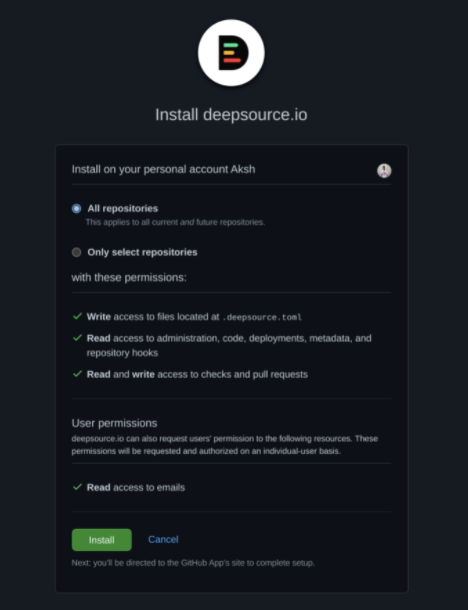
\includegraphics[scale=1.55]{figures/deepsource.png}
	\caption{ Установка приложения DeepSource на GitHub }\label{fig:deepsource}
\end{figure}

\begin{figure}[t!]
	\centering
	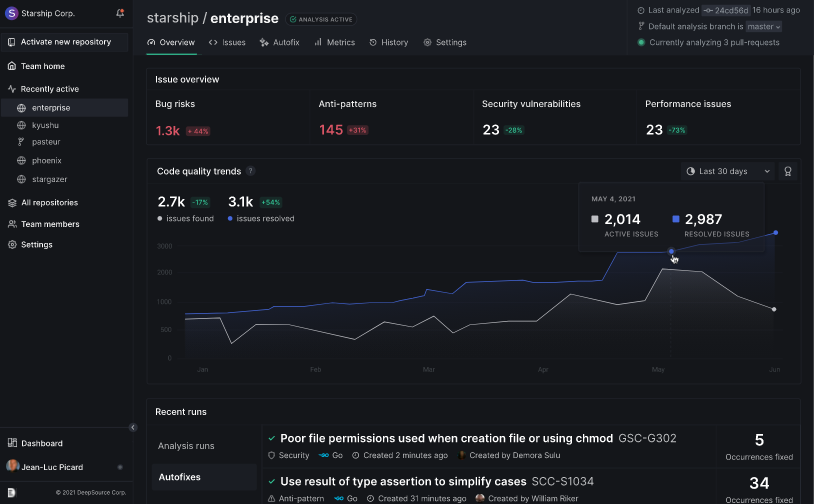
\includegraphics[scale=1.15]{figures/deepsource-dash.png}
	\caption{ Дешборд DeepSource }\label{fig:deepsource-dash}
\end{figure}

Аналогичным образом можно включать блоки для других поддерживаемых технологий и языков программирования. Например, для \texttt{Docker}
\begin{lstlisting}[
title = {\sffamily .deepsource (для Docker)},
style = bash,
numbers = none
]
version = 1

[[analyzers]]
name = "docker"
enabled = true

	[analyzers.meta]
	dockerfile_paths = [
		"dockerfile_dev",
		"dockerfile_prod"
	]

	trusted_registries = [
		"my-registry.com",
		"docker.io"
	]
...
\end{lstlisting}

Для SQL
\begin{lstlisting}[
title = {\sffamily .deepsource (для SQL)},
style = bash,
numbers = none
]
version = 1

[[analyzers]]
name = "sql"
enabled = true

	[analyzers.meta]
		max_line_length = 100
		tab_space_size = 4
		indent_unit = "tab"
		comma_style = "trailing"
		capitalisation_policy = "consistent"
		allow_scalar = true
		single_table_references = "consistent"
\end{lstlisting}

Для \texttt{Scala}
\begin{lstlisting}[
title = {\sffamily .deepsource (для Scala)},
style = bash,
numbers = none
]
version = 1

test_patterns = [
	"test/**",
	"*_test.scala"
]

exclude_patterns = [
	"vendor/**",
	"**/examples/**"
]

[[analyzers]]
name = "scala"
enabled = true
\end{lstlisting}

\subsection{Полезные ресурсы}

Документация проекта \texttt{deepsource.io}: \url{https://deepsource.io/}




%\listoffigures\addcontentsline{toc}{section}{Список иллюстраций}

% Источники в "Газовой промышленности" нумеруются по мере упоминания 
%\begin{thebibliography}{99}\addcontentsline{toc}{section}{Список литературы}
%	\bibitem{beazley:python-2010}{\emph{Бизли Д.} Python. Подробный справочник. -- Пер. с англ. -- СПб.: Символ-Плюс, 2010. -- 864~с. }
%\end{thebibliography}

\end{document}
